\section{Multivariate Analysis}
In our case the signal and background are not distinct, to seperate signal and background we need to find out the properties that distinct between the two. But, there does not exists any variable that can distinguish clearly the signal and background. So, we tried to use the multivariate techniques to see how much it can imporve our analysis. So, we did few different types of traning and check how much we can gain as compared to the cut based analysis. At the end of this section results are summarized.

%
%	Why we are going to use BDT not DNN, kNN, etc?
%


%
%	Why DT with Gradient Boost?
%

%
%	List of traning done and its result
%
%\section{Details of BDT analysis}
\subsection{Traning 1}
Some basic information for the BDT traning are
\begin{itemize}
	\item BDT is optimized for aQGC signal only not for SM. As for SM we don't have enough statistics for traning.
	\item aQGC point considered is -0.4$\times 10^{-12}$ TeV$^{-4}$
	\item For traning considered backgrounds are
	\begin{itemize}
		\item WWJJ QCD
		\item W+jets HT-binned sample
		\item TTbar, Single tops, TTW, and TTZ
	\end{itemize}
\end{itemize}
List of input variables used are:
\begin{enumerate}
	\item lepton $p_T$, $\eta$
	\item Leptonic W $p_T$, $\eta$, transverse mass ($m_T$)
	\item pfMET (type I corrected)
	\item AK8 jet invariant mass, $p_T$, $\eta$
	\item Four body invairant mass, $p_T$, $\eta$
	\item number of AK4 jets (passed $p_T$ requirement and cleaned from leptons and AK8 jets only).
	\item Selected VBF jets $p_T$, $\eta$
	\item VBF di-jet invariant mass
	\item difference between $\eta$ of two VBF jets.
	\item difference in azimuthal angle between selected AK8 jet and pfMET
	\item Angular variables (cos($\theta^*$), cos($\theta 1$), cos($\theta 2$), $\phi$, and $\phi 1$   )
	\item Boson centrality
	\item $p_T$ balance
	\item leptonic and hadronic zeppenfeld
\end{enumerate}


List of traning cuts are:
\begin{itemize}
	\item Exactly one lepton having
	\begin{itemize}
		\item $p_T > 30$ GeV
		\item $|\eta| < 2.4$
	\end{itemize}
	\item pfMET $>$ 50 GeV
	\item AK8 jets
	\begin{itemize}
		\item  p$_T >$ 200 GeV
		\item $|\eta|<2.4$
		\item $\tau 21 < 0.55$
		\item 40$<$mW$<$150
	\end{itemize}
	\item Loose AK4 b-tagged jet veto
	\begin{itemize}
		\item $p_T>30$ GeV
		\item $m_{jj}>500$ GeV
	\end{itemize}
\end{itemize}

\subsubsection{BDT performance summary}

\begin{figure}[h!]
	 \centering
	 \subfigure[]{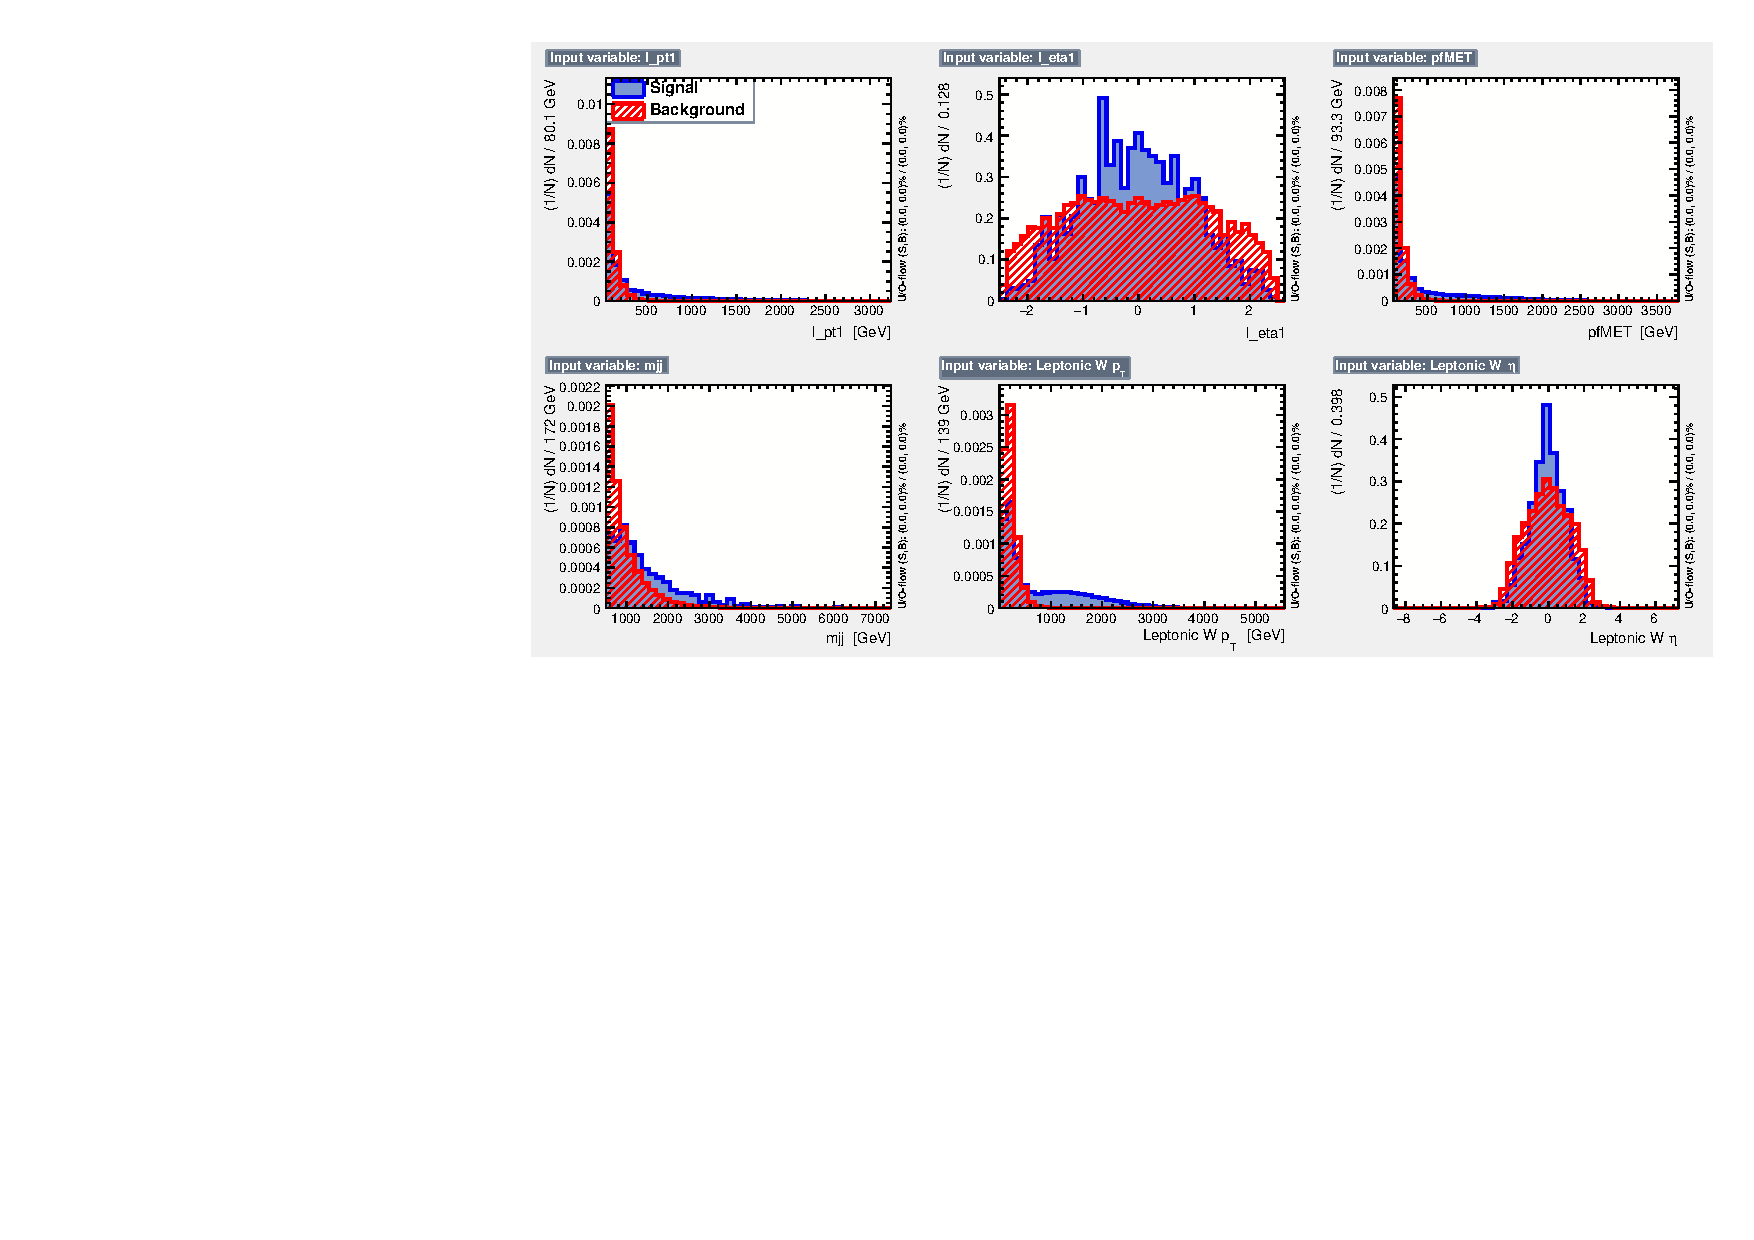
\includegraphics[scale=0.85]{Plots/BDT_Performance/Trial1/dataset/plots/canvas1.pdf}}
	 \caption{Signal-background comparison; Top (From left to right): lepton $p_T$, lepton $\eta$, MET; Bottom (From left to right): VBF di-jet invariant mass, leptonic W transverse momentum, leptonic W $\eta$ }
\end{figure}
\begin{figure}[h!]\ContinuedFloat
	 \subfigure[]{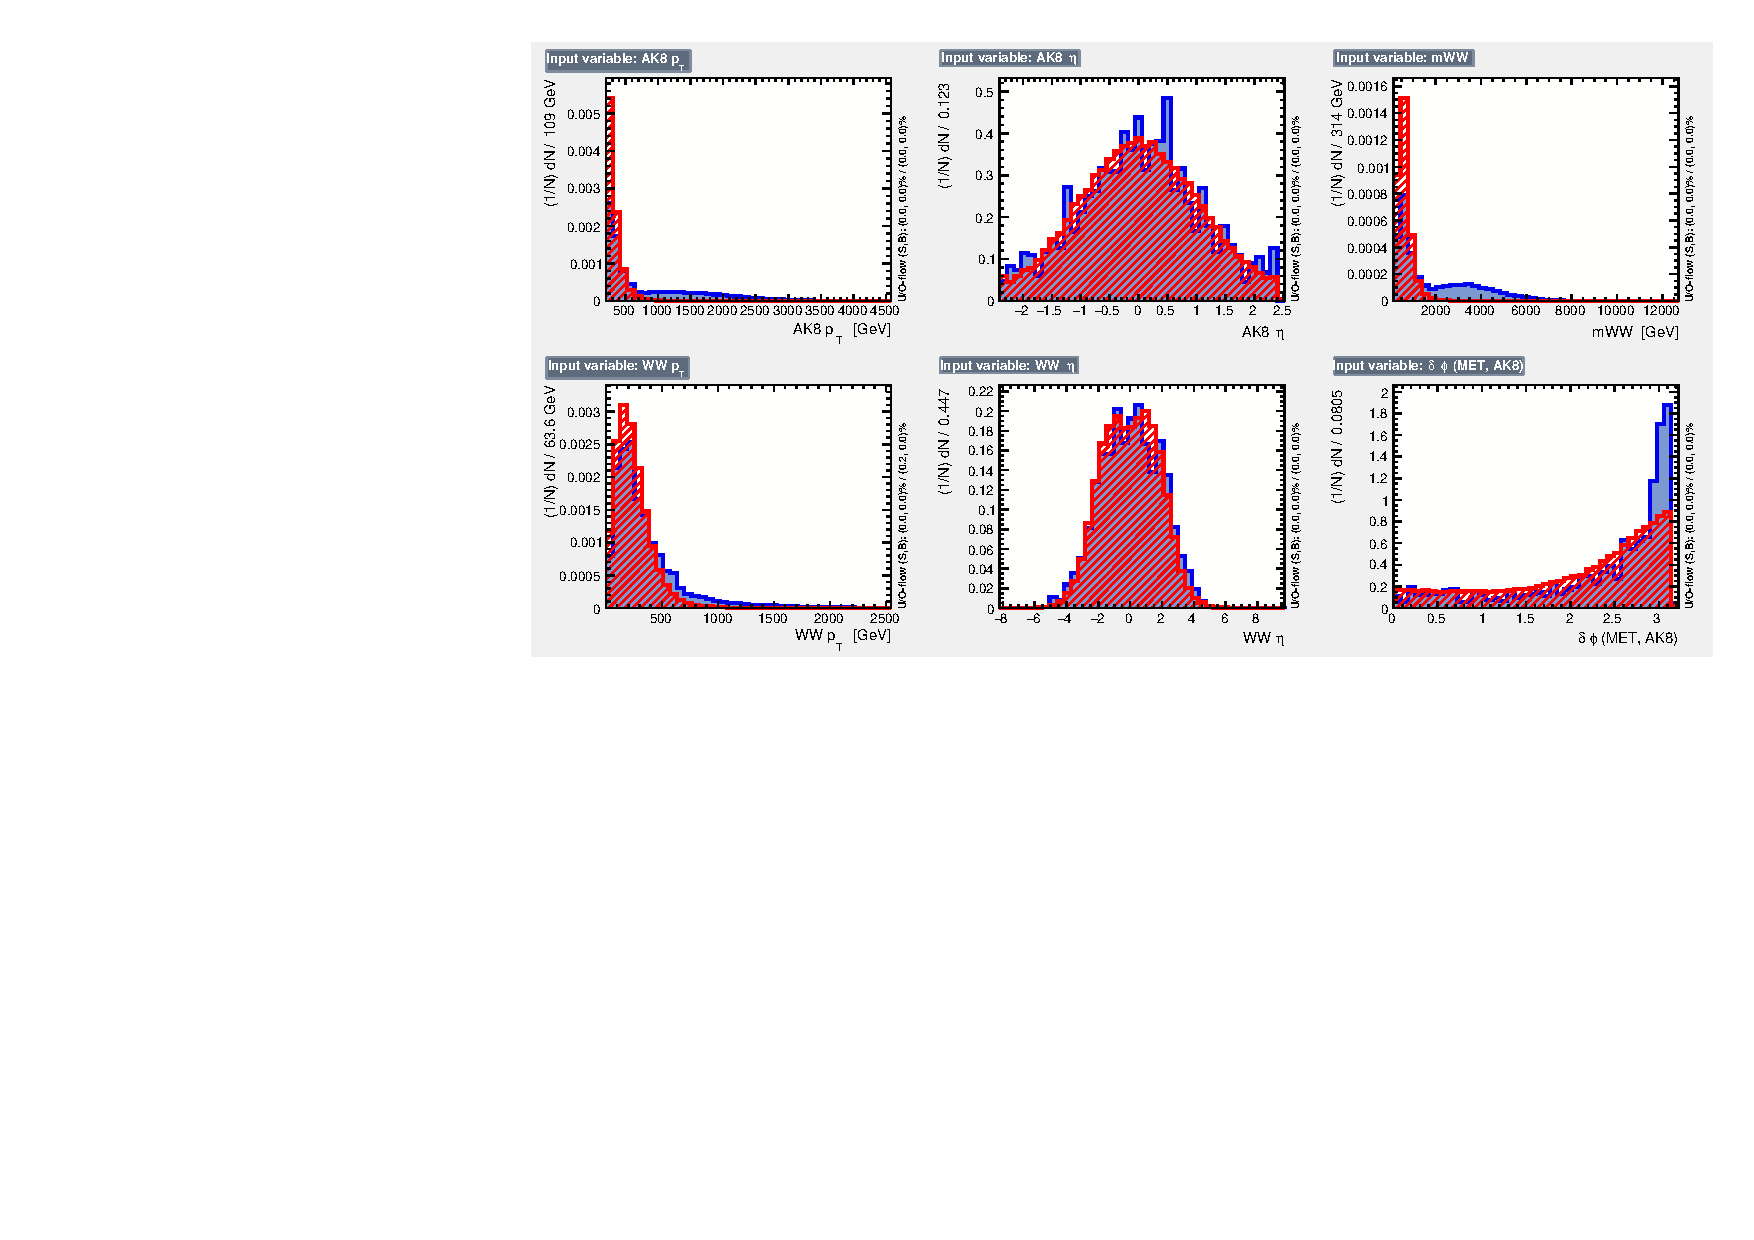
\includegraphics[scale=0.85]{Plots/BDT_Performance/Trial1/dataset/plots/canvas2.pdf}}
	\caption{Signal-background comparison; Top (From left to right): AK8 jet $p_T$, AK8 jet $\eta$, invariant mass of WW system; Bottom (From left to right): WW system $p_T$, WW system $\eta$, $\delta \phi (MET, AK8 jet)$}
\end{figure}
\begin{figure}[h!]\ContinuedFloat
	 \subfigure[]{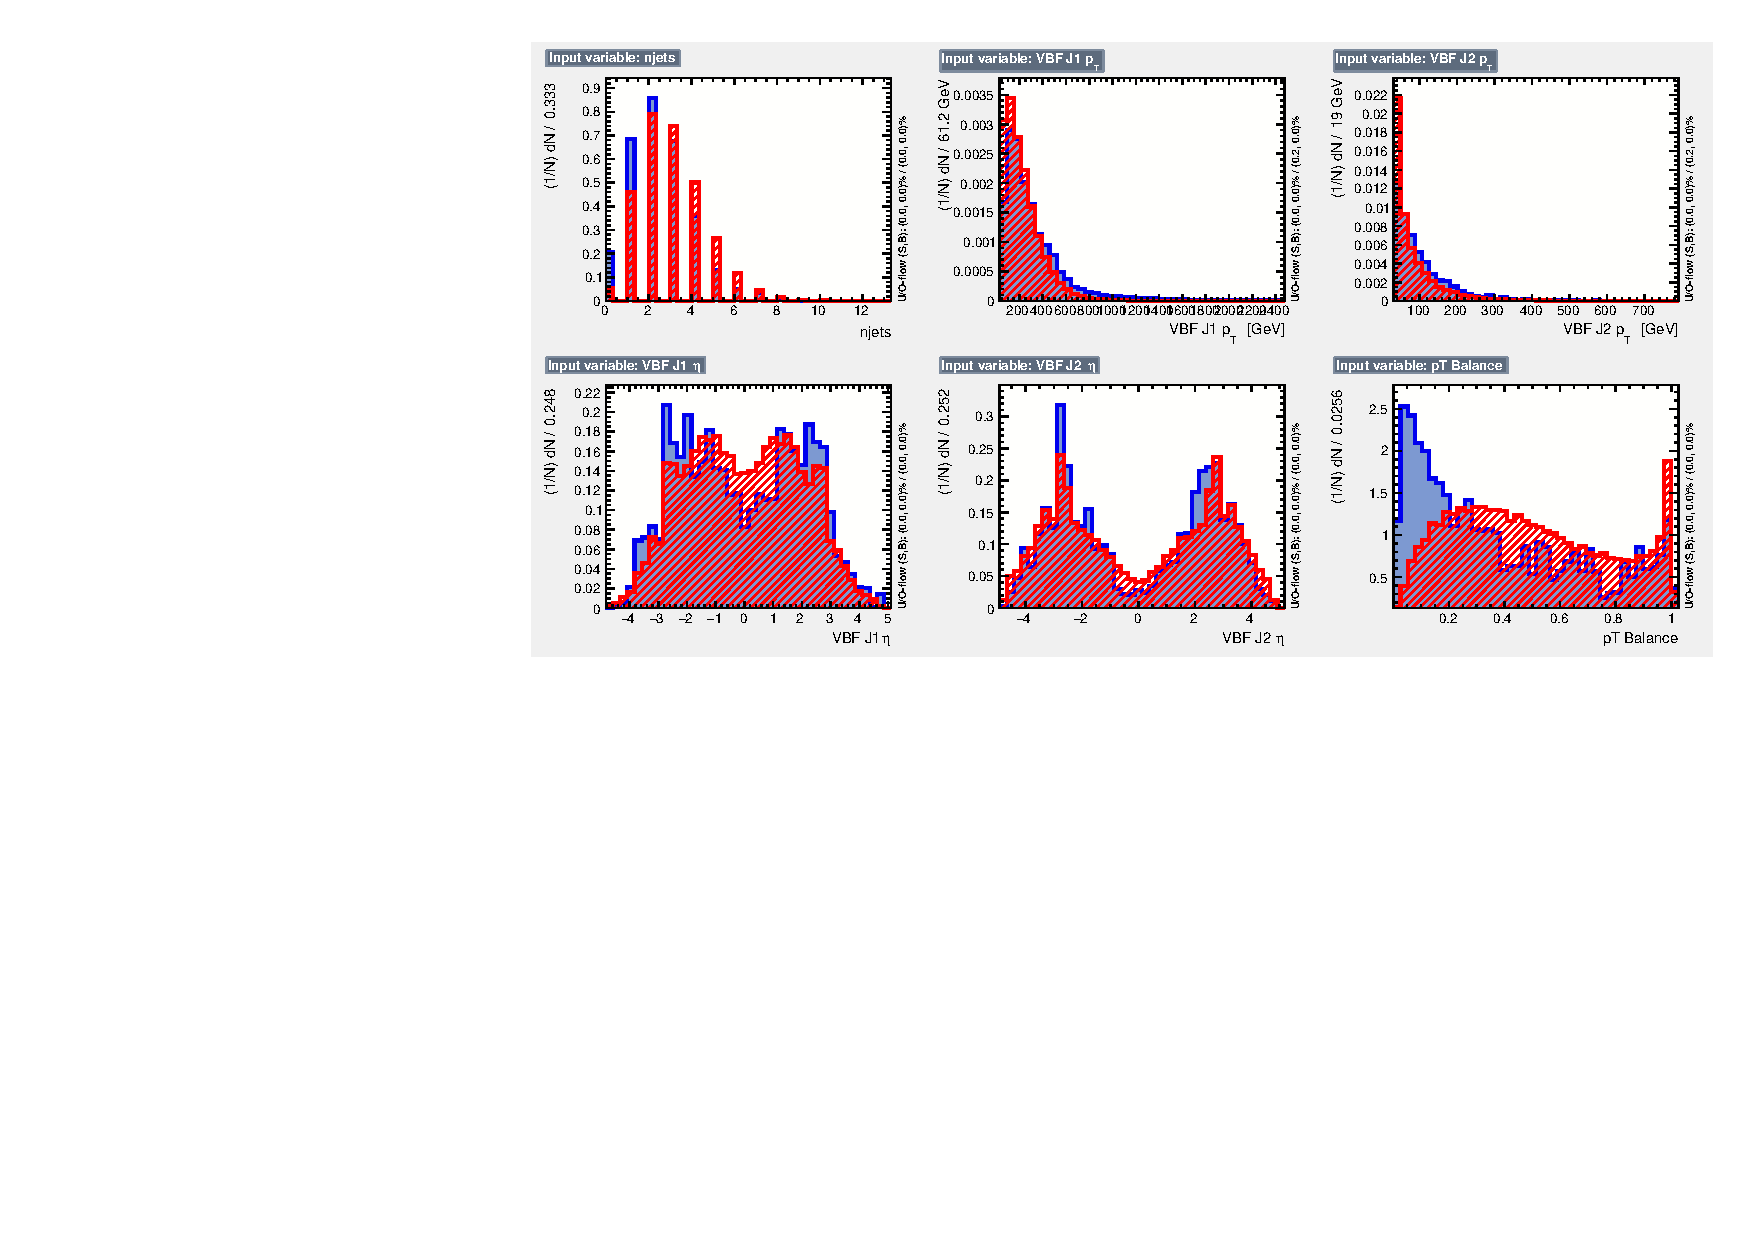
\includegraphics[scale=0.85]{Plots/BDT_Performance/Trial1/dataset/plots/canvas3.pdf}}
	 \caption{Signal-background comparison; Top (From left to right): Number of AK4 jets passing $p_T$ cut and cleaned from lepton and AK8 jets, leading VBF jet $p_T$, sub-leading VBF jet $p_T$; Bottom (From left to right): leading VBF jet $\eta$, sub-leading VBF jet $\eta$, $p_T$ balance (as defined in Eq.~\ref{eq:ptBalance})}
\end{figure}
\begin{figure}[h!]\ContinuedFloat
	 \subfigure[]{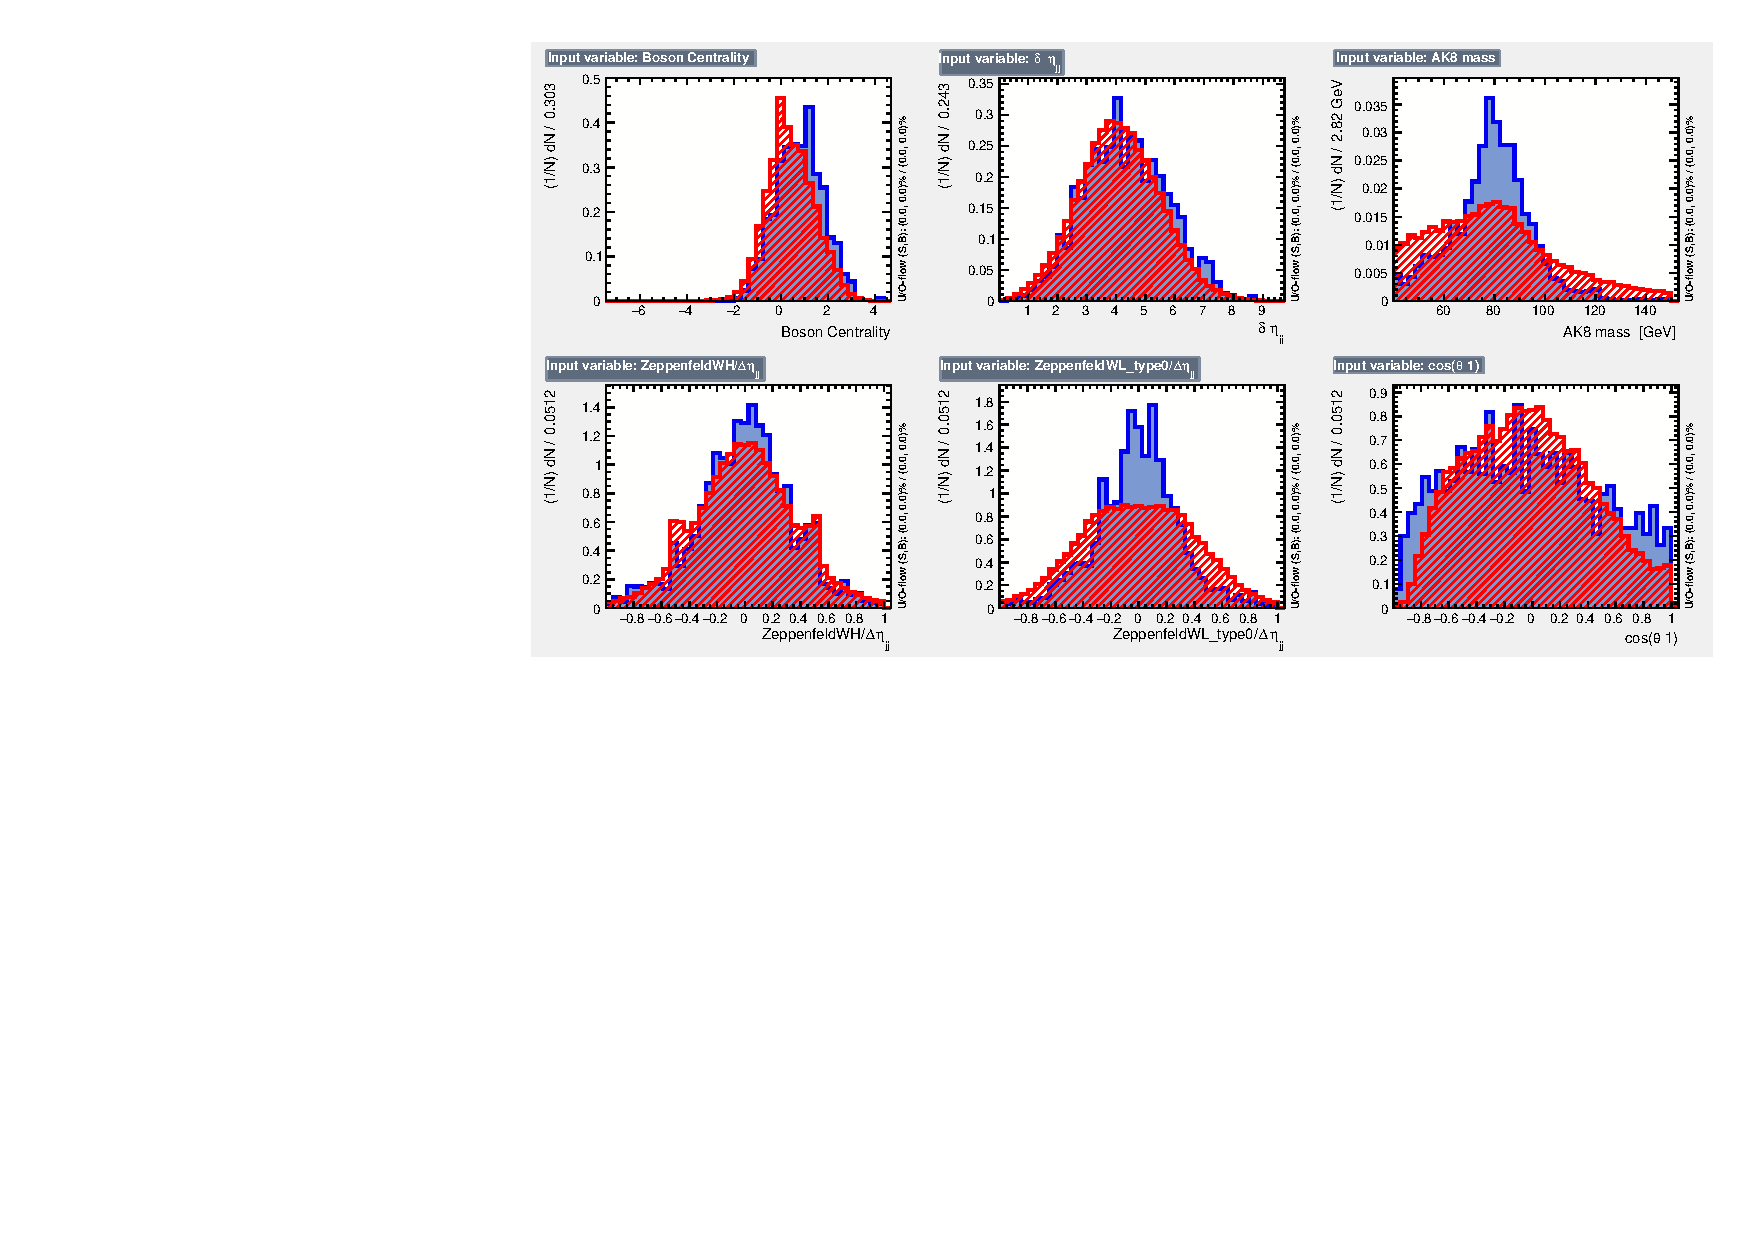
\includegraphics[scale=0.85]{Plots/BDT_Performance/Trial1/dataset/plots/canvas4.pdf}}
	 \caption{Signal-background comparison; Top (From left to right): boson centrality (as defined in Eq.~\ref{eq:bosonCentrality}), pseudo-rapidity gap between VBF jets, AK8 jet invariant mass; Bottom (From left to right): Hadronic zeppenfeld (as defined in Eq.~\ref{eq:HadZep}), Leptonic zeppenfeld (as defined in Eq.~\ref{eq:LepZep}), cos($\theta_1$) (one of angular variable)}
\end{figure}
\begin{figure}[h!]\ContinuedFloat
	 \subfigure[]{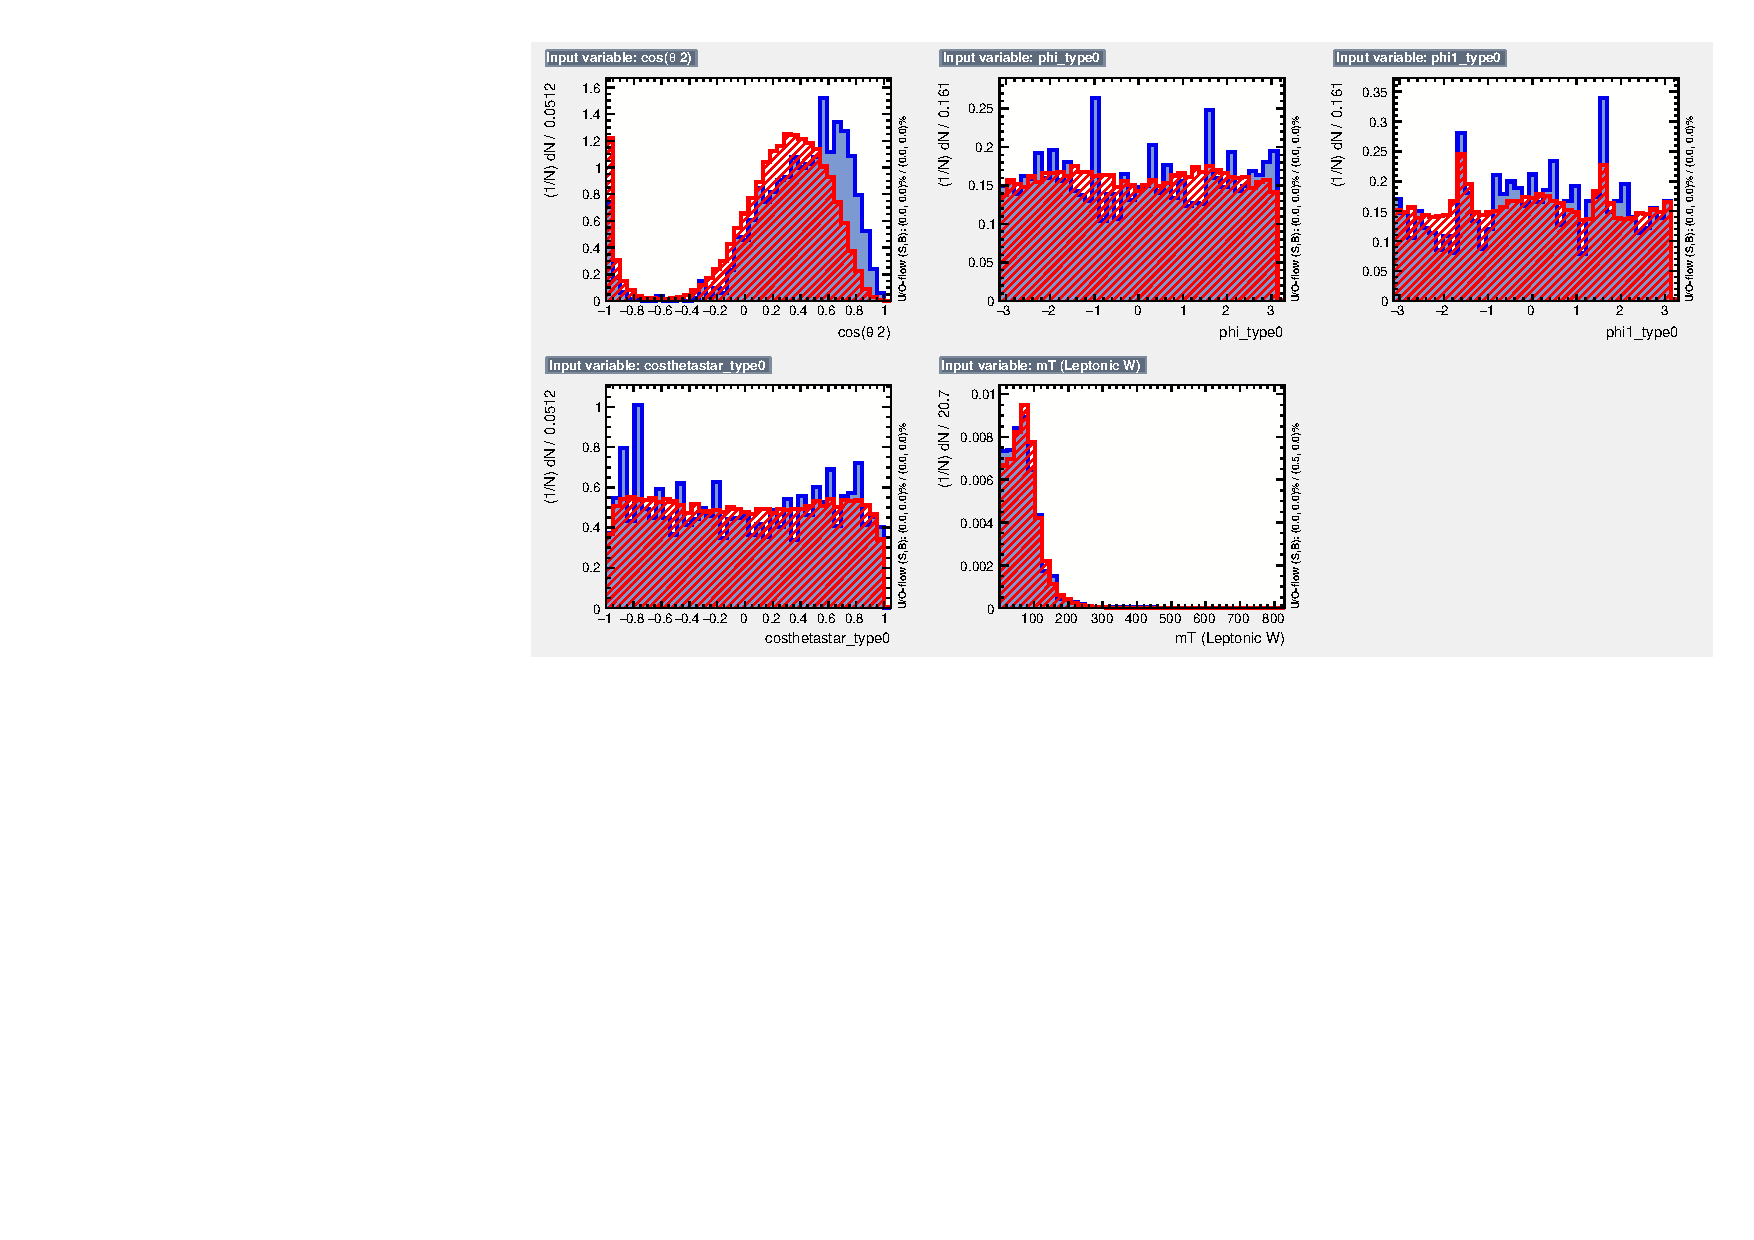
\includegraphics[scale=0.85]{Plots/BDT_Performance/Trial1/dataset/plots/canvas5.pdf}}
	 \caption{Signal-background comparison; Top (From left to right):cos($\theta_2$), $\phi$, $\phi_1$  ; Bottom (From left to right): cos$\theta^{\ast}$, transverse mass of leptonic decayed W-boson}
\end{figure}

\clearpage
\subsubsection{Overtraning Check}
\begin{figure}[h!]
	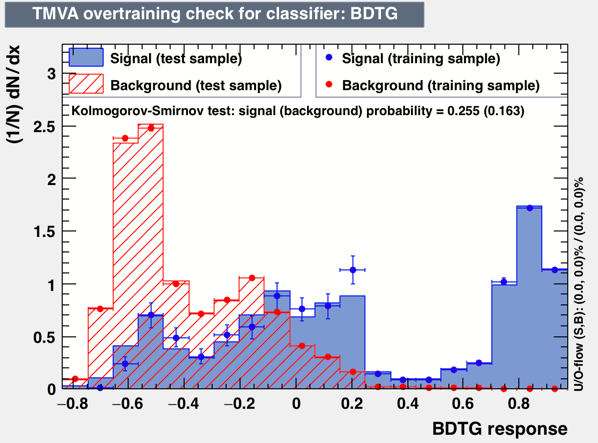
\includegraphics[scale=0.40]{Plots/BDT_Performance/Trial1/dataset/plots/overtrain_BDTG.png}%
	~
	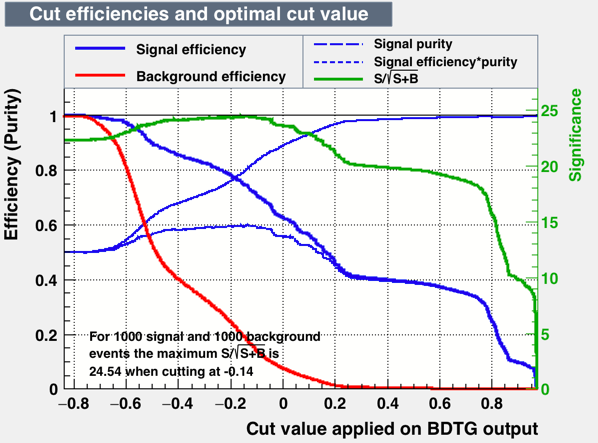
\includegraphics[scale=0.40]{Plots/BDT_Performance/Trial1/dataset/plots/mvaeffs_BDTG.png}
	\caption{Left: Traning and test distribuion for output of BDT response; Right: Cut efficiency and significance for BDT response}
\end{figure}

\begin{figure}[h!]
	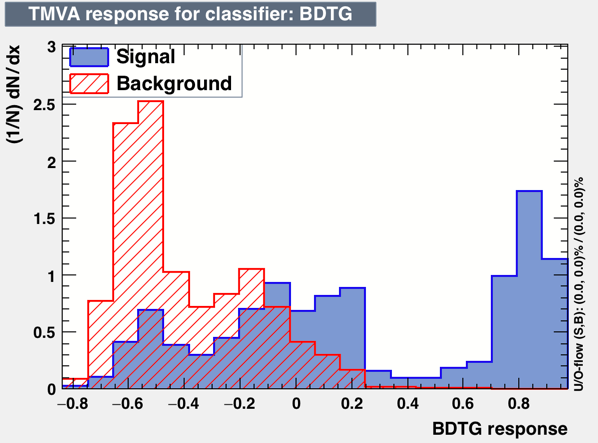
\includegraphics[scale=0.40]{Plots/BDT_Performance/Trial1/dataset/plots/mva_BDTG.png}%
	~
	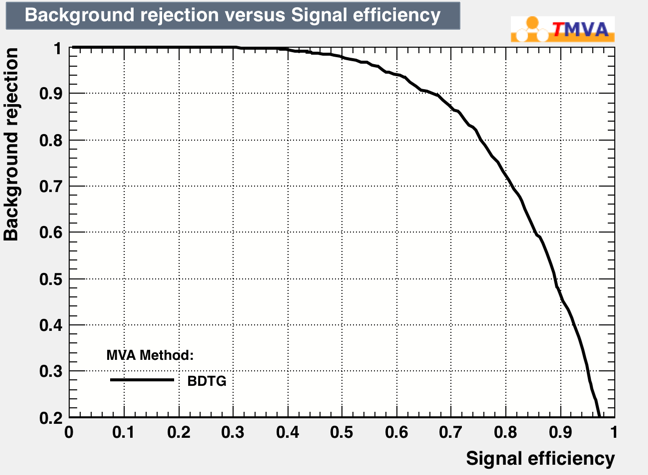
\includegraphics[scale=0.40]{Plots/BDT_Performance/Trial1/dataset/plots/rejBvsS.png}
	\caption{Left: BDT response for signal and background; Right: ROC curve}
\end{figure}

\begin{figure}[h!]
	 \centering
	 \subfigure[]{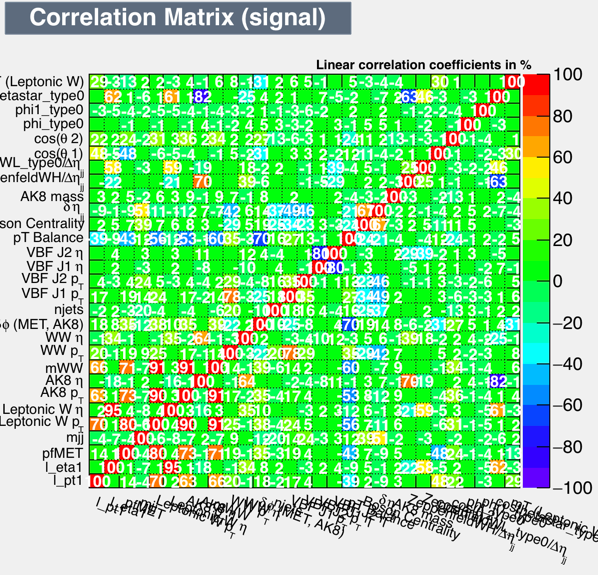
\includegraphics[width=1.2\textwidth, angle =90]{Plots/BDT_Performance/Trial1/dataset/plots/CorrelationMatrixS.png}}
	 \caption{Correlation plot for signal}
\end{figure}
\begin{figure}[h!]\ContinuedFloat
	 \subfigure[]{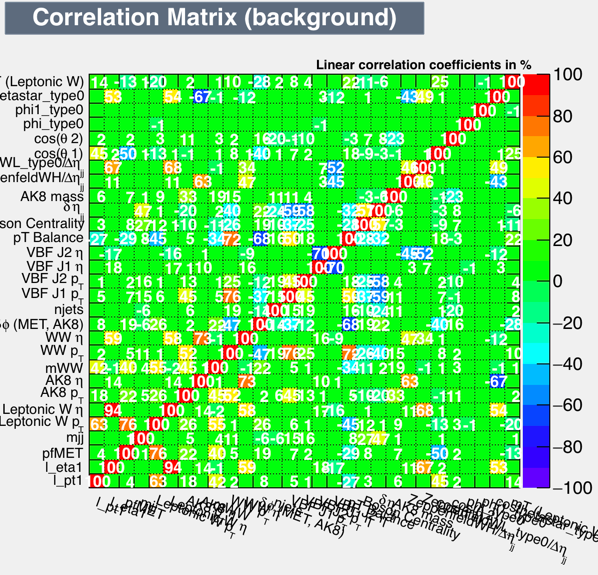
\includegraphics[width=1.2\textwidth, angle =90]{Plots/BDT_Performance/Trial1/dataset/plots/CorrelationMatrixB.png}}
	 \caption{Correlation plot for background}
\end{figure}
%\input{InputVariables.tex}
%
%	Comparison of BDT with simple cut based
%
\clearpage
\subsubsection{Check the modeling of BDT variable}
To check the modeling of the BDT variables we will try to make the Wjet and TTbar control region with the BDT cut only and check its distribution.
\begin{figure}[ht!] 
	 \centering
	 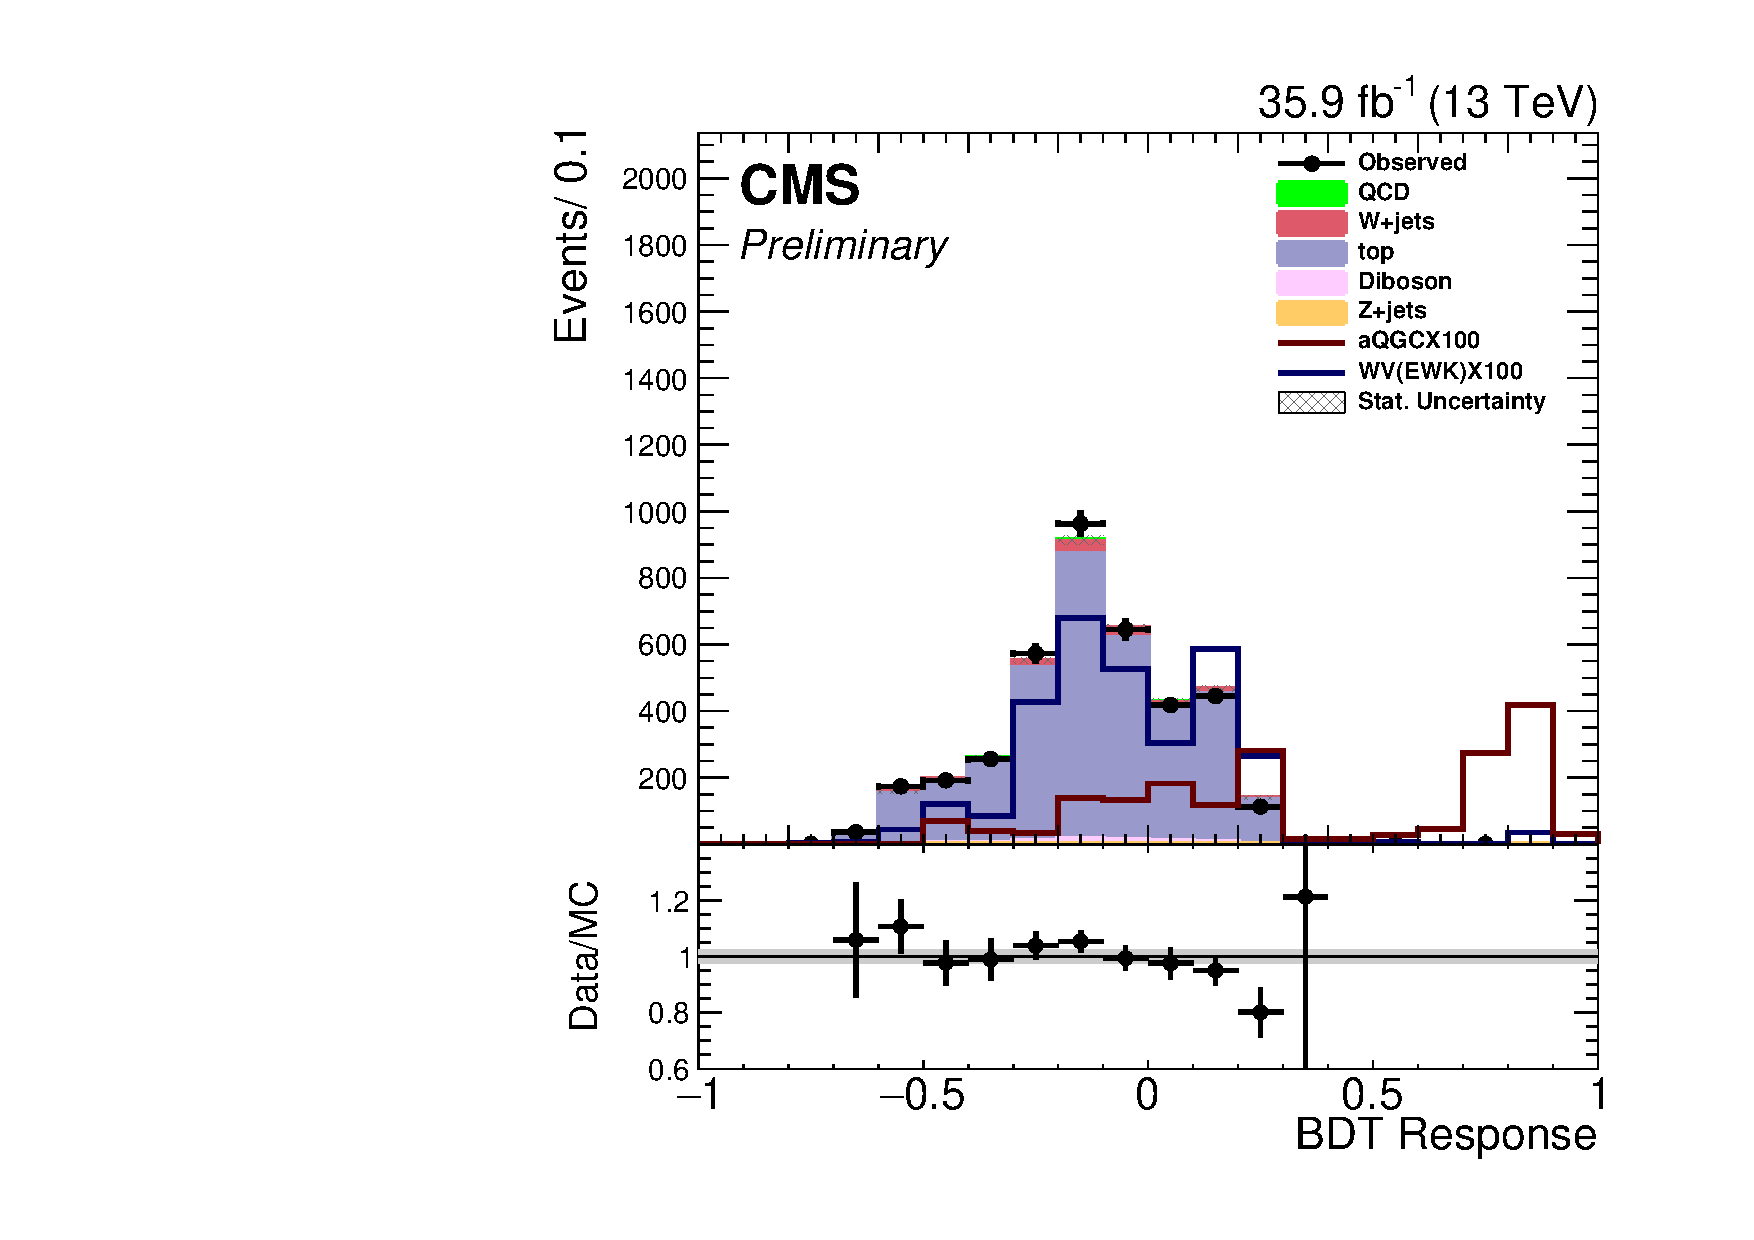
\includegraphics[scale=0.38]{Plots/ControlPlots/BDT/DibosonBoostedElMuCuts13TeV_TTBarControlRegion_CHS_BDT_response.pdf}%
	 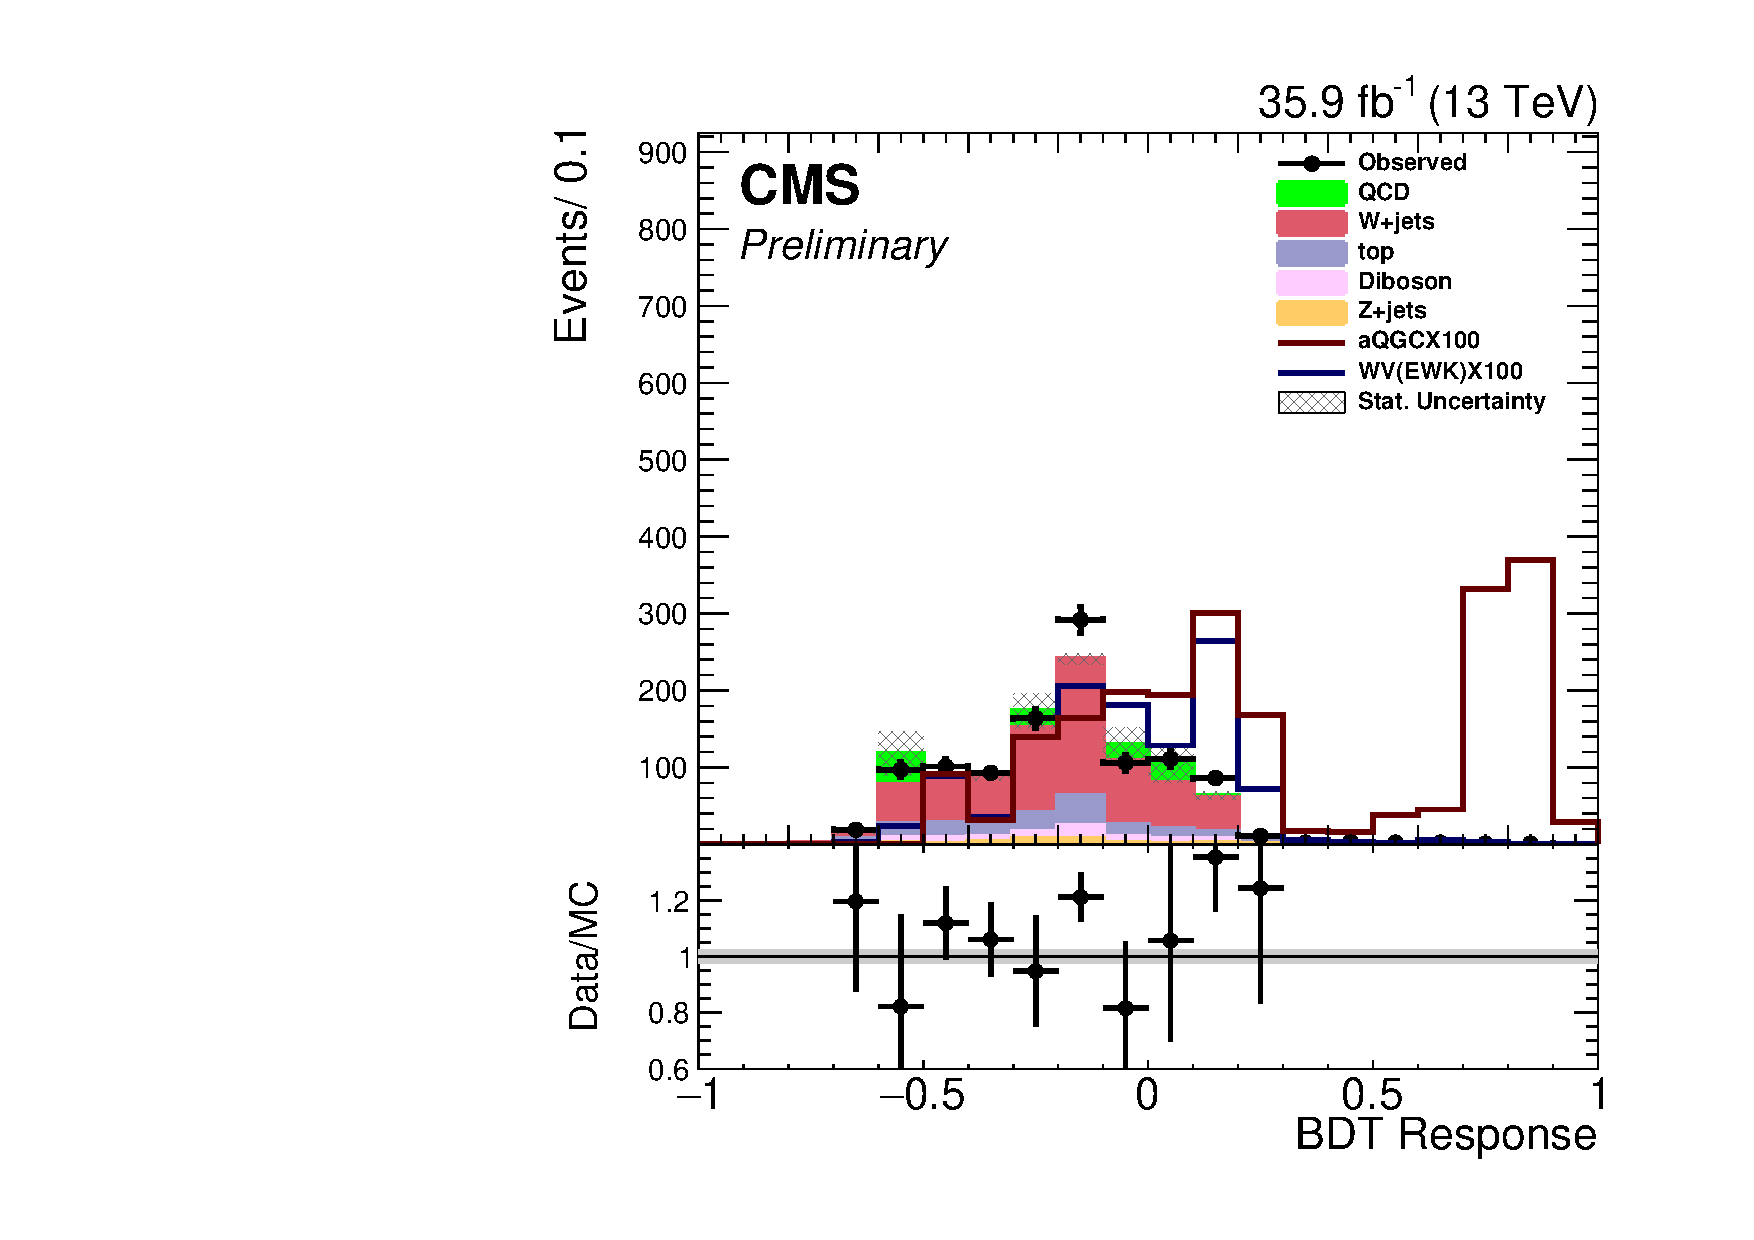
\includegraphics[scale=0.38]{Plots/ControlPlots/BDT/DibosonBoostedElMuCuts13TeV_WjetControlRegion_Tighter_CHS_BDT_response.pdf}
	 \caption{Left: TTbar control region for BDT response. Right: Wjet control region for BDT response}
	 \label{fig:BDT_response_modeling}
\end{figure}

\subsubsection{Significance from combine}
The combine card is
\begin{verbatim}
----------------------------------------------------------
imax 1 number of channels
jmax * number of background
kmax * number of nuisance parameters
---------------------------------------------------------
shapes * * Nominal.root $PROCESS $PROCESS_$SYSTEMATIC
shapes data_obs * Nominal.root data
----------------------------------------------------------
Observation -1
bin WV WV WV WV WV
----------------------------------------------------------
process top W+jets Z+jets Diboson aQGC
process 1 2 3 4 0
rate -1.00000 -1.00000  -1.00000  -1.00000  -1.00000  
----------------------------------------------------------
lumi_13TeV			lnN	1.027	1.027	1.027	1.027	1.02700  
norm_Wjet 			lnN	-		1.100	-		-		-  
CMS_eff_b_mistag	lnN	0.980	0.980	0.98	0.980	0.98000
CMS_eff_m      		lnN	1.018	1.018	1.018	1.018	1.01800
CMS_eff_e      		lnN	1.017	1.017	1.017	1.017	1.01700
ewk_qqbar      		lnN	-		-		-		-		1.15000   
norm_top          	lnN	1.10	-		-		-		-  
----------------------------------------------------------
\end{verbatim}

Significance we get with BDT observable is 9.60994.

The distribution for the BDT observable is 
\begin{figure}[htb]
  \begin{center}
    \begin{tabular}{c}
    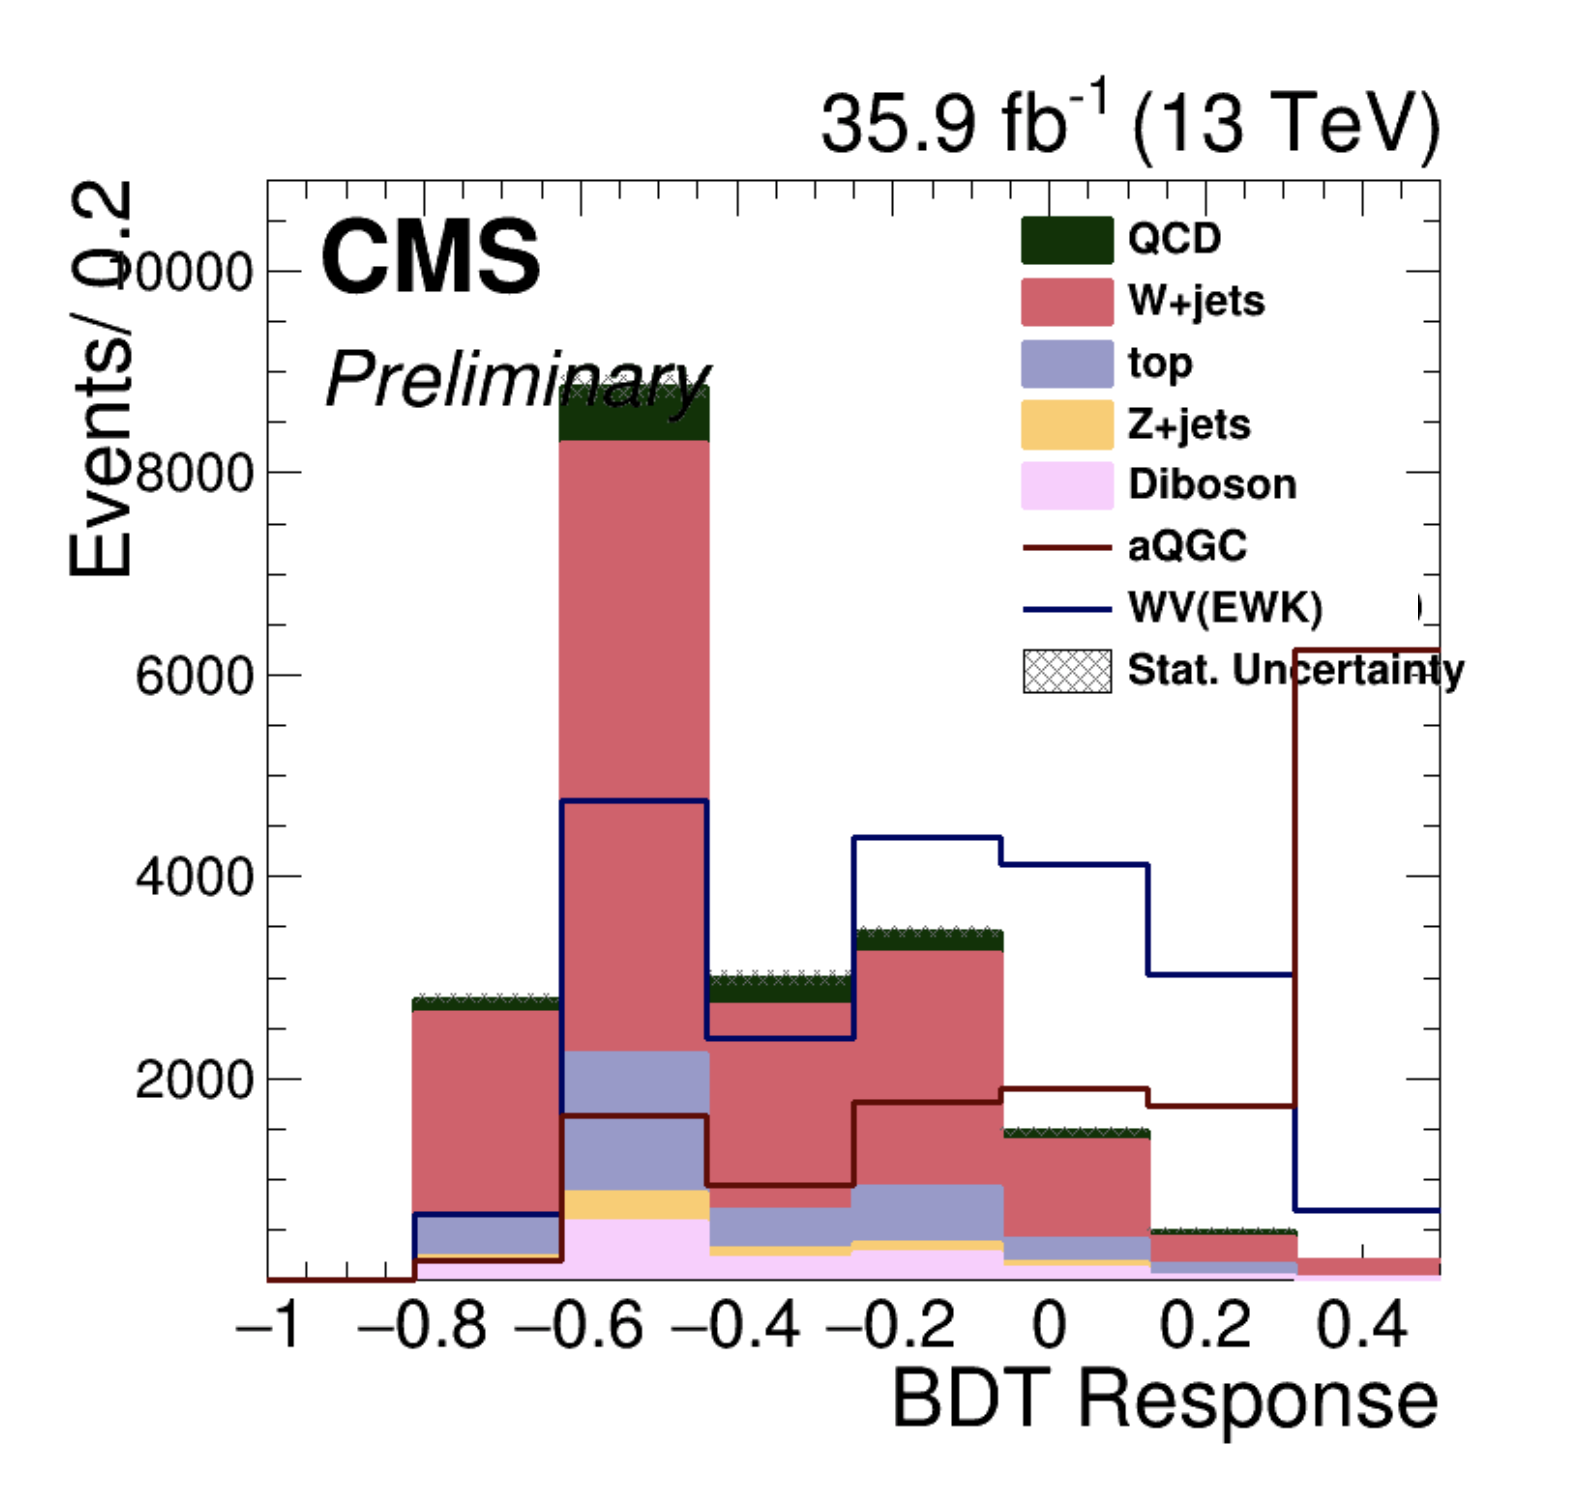
\includegraphics[width=0.90\textwidth]{Plots/BDT_Performance/Trial1/BDT_observable.png}    
    \end{tabular}
    \caption{BDT distribution. This is our observable.}
    \label{fig:gen1}
  \end{center}
\end{figure}


\clearpage
\subsection{Traning 2}
List of input variables used are:
\begin{enumerate}
	\item lepton $\eta$
	\item Four body $\eta$
	\item difference in azimuthal angle between selected AK8 jet and pfMET
	\item Angular variables (cos($\theta^*$), cos($\theta 1$), cos($\theta 2$), $\phi$, and $\phi 1$   )
	\item Boson centrality
	\item $p_T$ balance
	\item leptonic and hadronic zeppenfeld
\end{enumerate}


List of traning cuts are:
\begin{itemize}
	\item Exactly one lepton having
	\begin{itemize}
		\item $p_T > 30$ GeV
		\item $|\eta| < 2.4$
	\end{itemize}
	\item pfMET $>$ 50 GeV
	\item AK8 jets
	\begin{itemize}
		\item  p$_T >$ 200 GeV
		\item $|\eta|<2.4$
		\item $\tau 21 < 0.55$
		\item 65$<$mW$<$105
	\end{itemize}
	\item Loose AK4 b-tagged jet veto
	\begin{itemize}
		\item $p_T>30$ GeV
		\item $m_{jj}>500$ GeV
	\end{itemize}
\end{itemize}

\subsubsection{BDT performance summary}


\begin{figure}[h!]
	 \centering
	 \subfigure[]{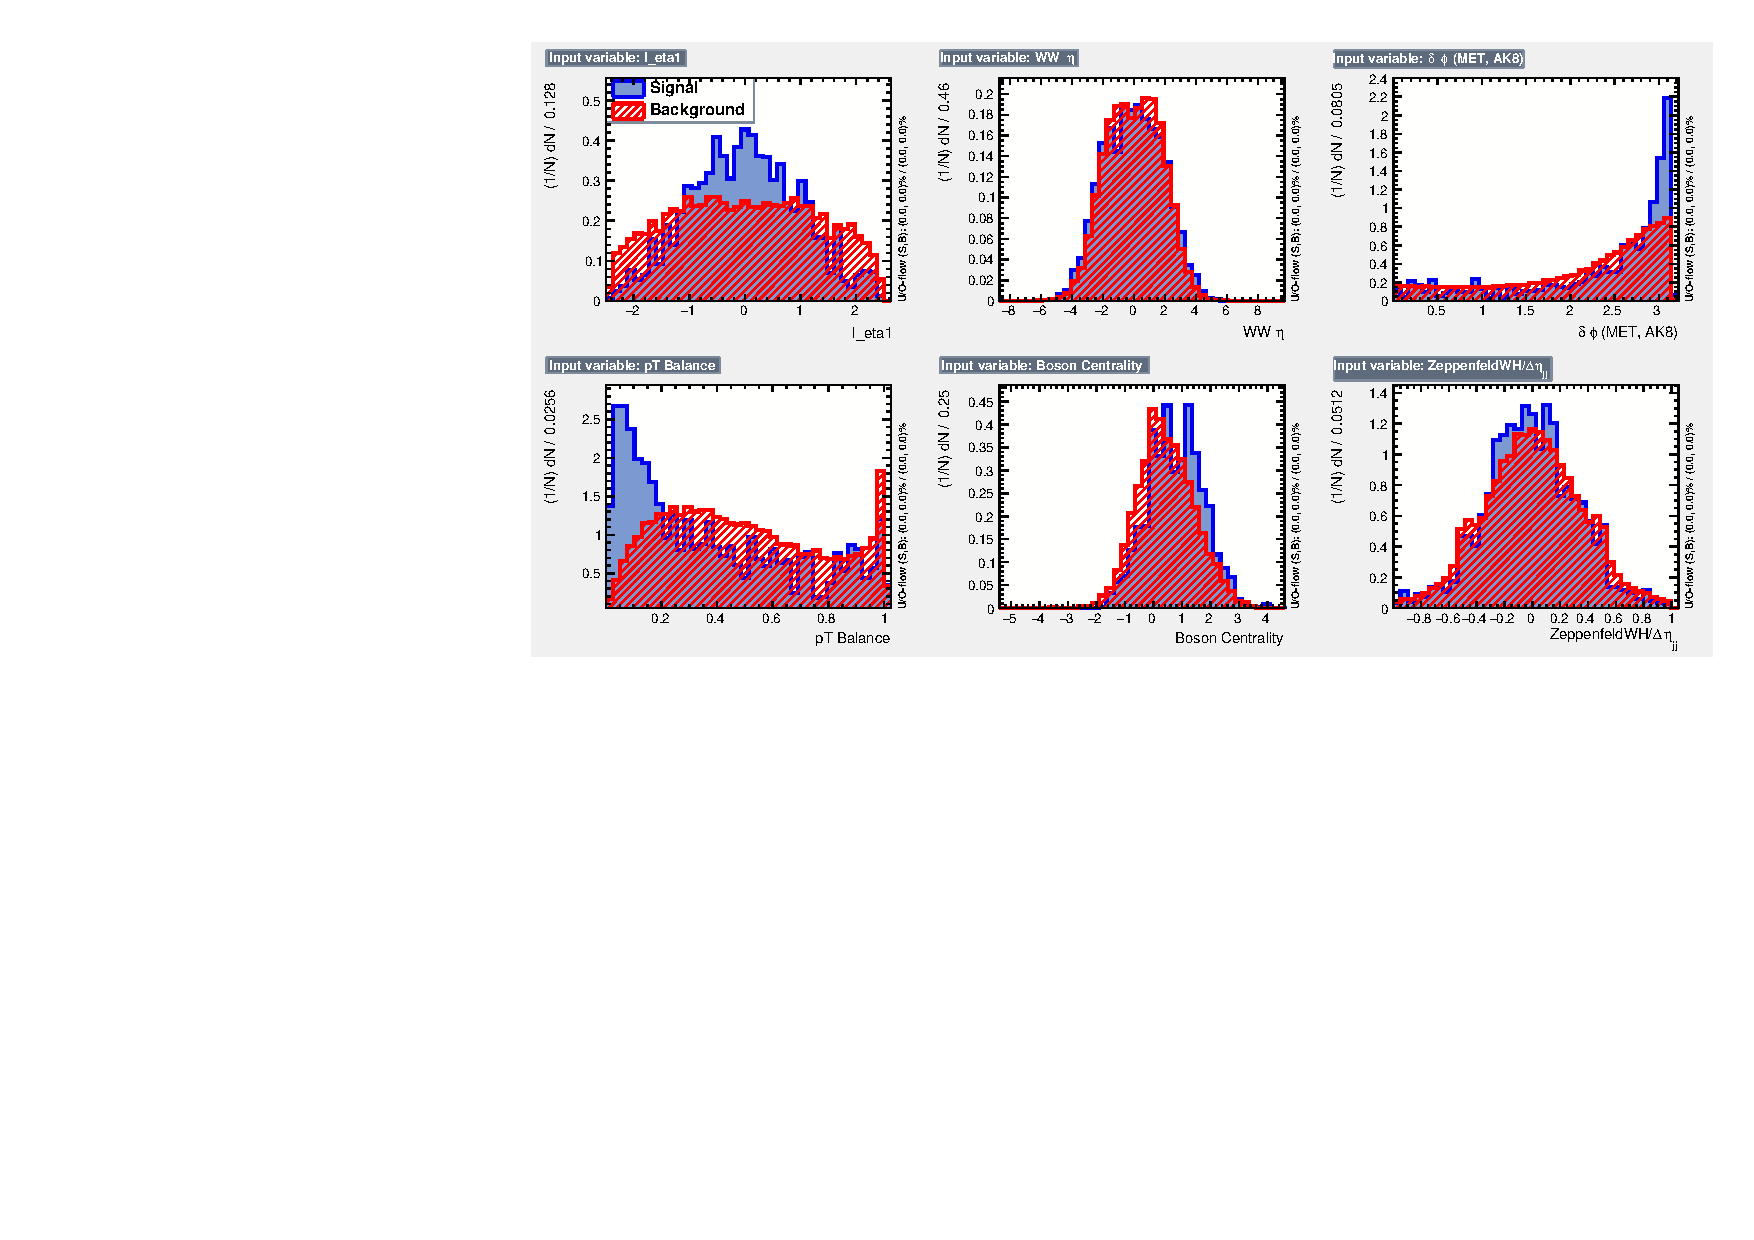
\includegraphics[scale=0.85]{Plots/BDT_Performance/Trial2/dataset/plots/canvas1.pdf}}
	 \caption{Signal-background comparison; Top (From left to right): lepton $\eta$, WW system $\eta$, $\delta \phi (MET, AK8 jet)$ ; Bottom (From left to right): $p_T$ balance (as defined in Eq.~\ref{eq:ptBalance}), boson centrality (as defined in Eq.~\ref{eq:bosonCentrality}), Hadronic zeppenfeld (as defined in Eq.~\ref{eq:HadZep})}
\end{figure}
\begin{figure}[h!]\ContinuedFloat
	 \subfigure[]{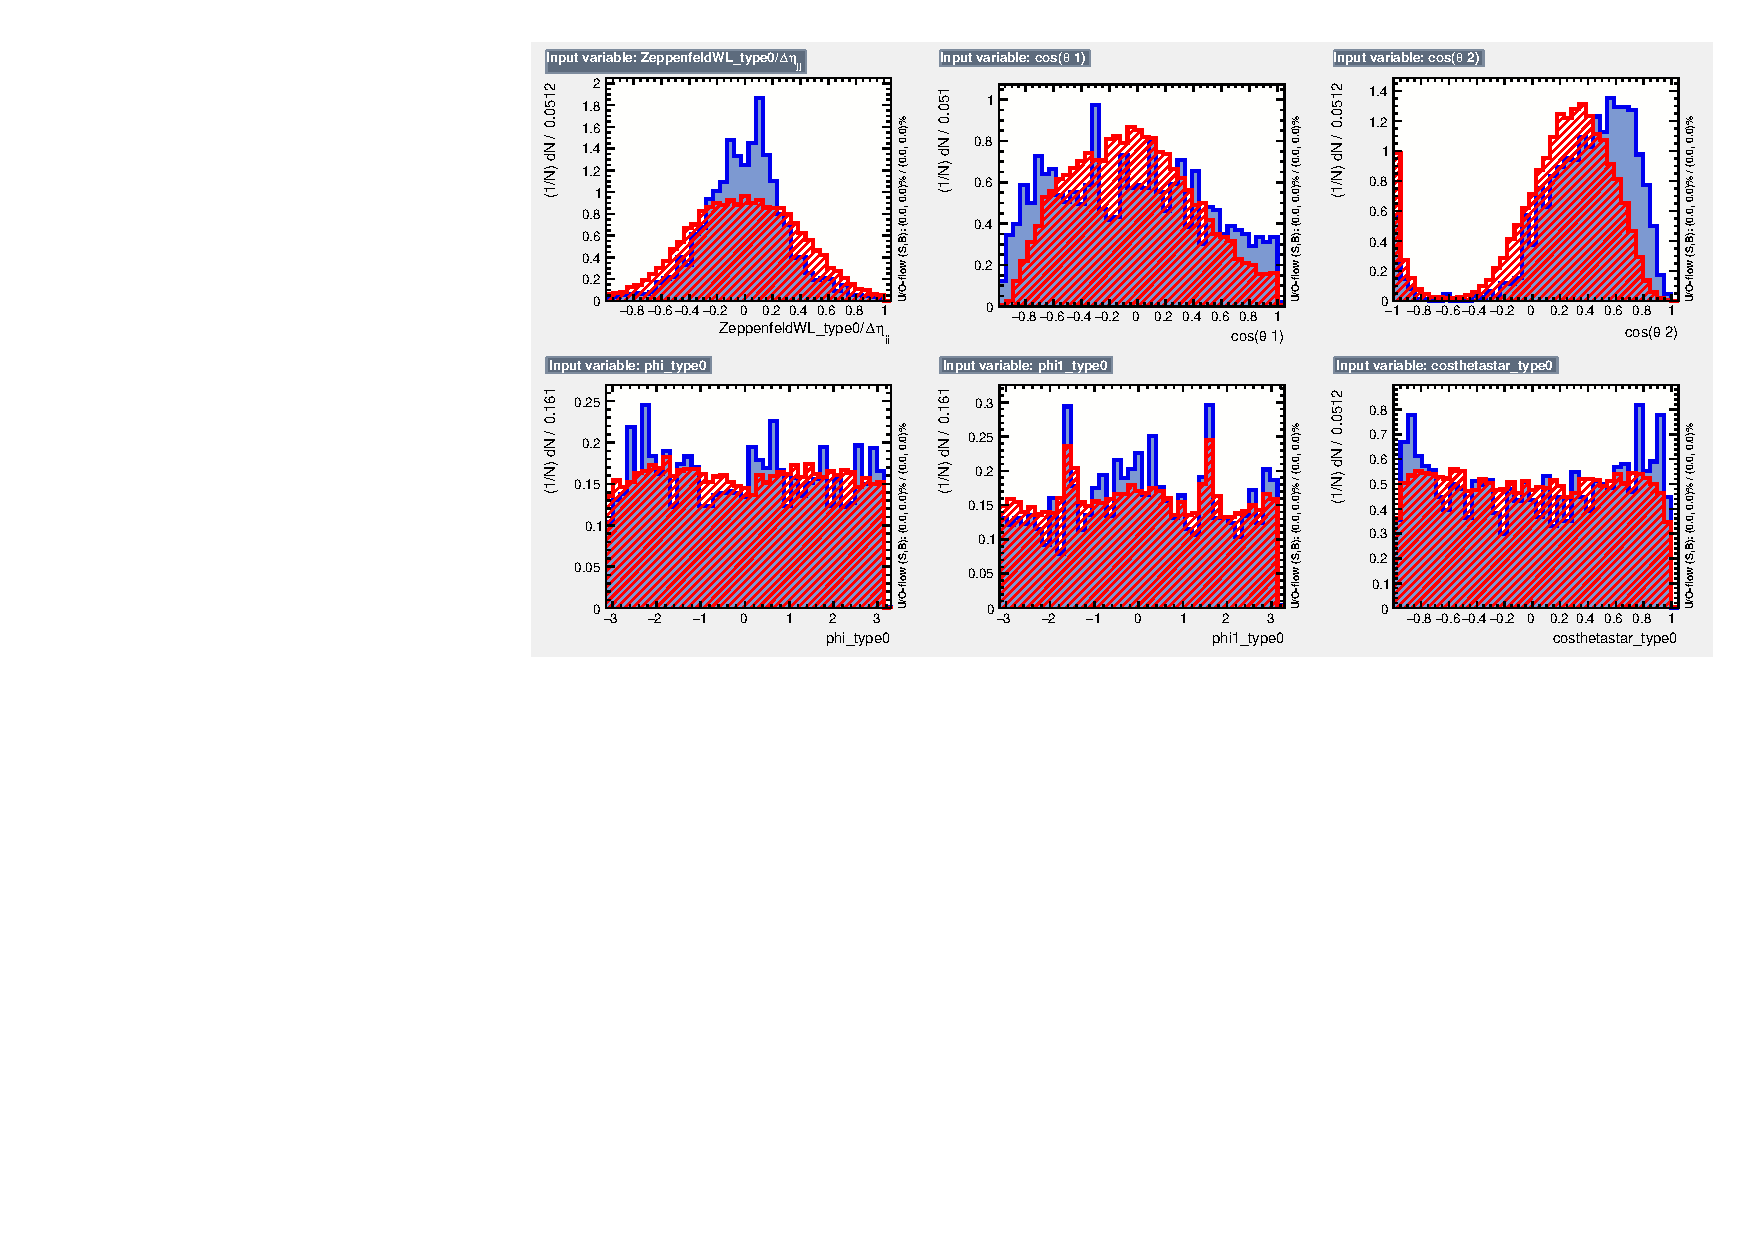
\includegraphics[scale=0.85]{Plots/BDT_Performance/Trial2/dataset/plots/canvas2.pdf}}
	 \caption{Signal-background comparison; Top (From left to right): Leptonic zeppenfeld (as defined in Eq.~\ref{eq:LepZep}), cos($\theta_1$) and cos($\theta_2$); Bottom (From left to right): $\phi$, $\phi_1$ and cos$\theta^{\ast}$ }
\end{figure}

\clearpage
\subsubsection{Overtraning Check}
\begin{figure}[h!]
	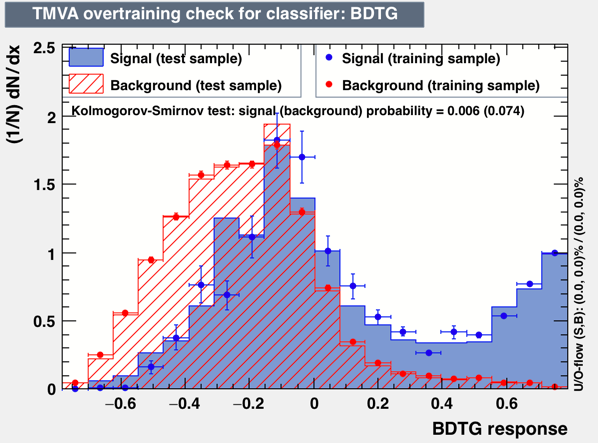
\includegraphics[scale=0.40]{Plots/BDT_Performance/Trial2/dataset/plots/overtrain_BDTG.png}%
	~
	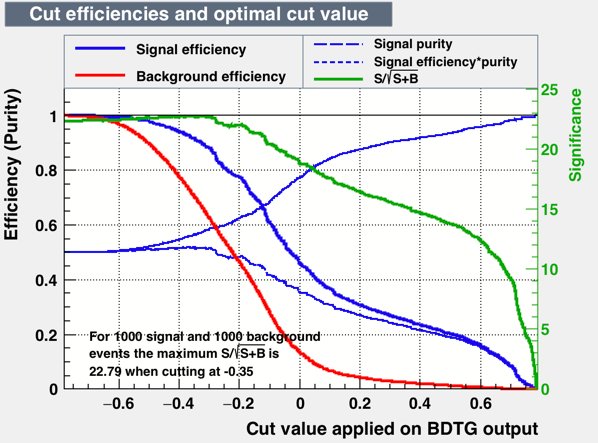
\includegraphics[scale=0.40]{Plots/BDT_Performance/Trial2/dataset/plots/mvaeffs_BDTG.png}
	\caption{Left: Traning and test distribuion for output of BDT response; Right: Cut efficiency and significance for BDT response}
\end{figure}

\begin{figure}[h!]
	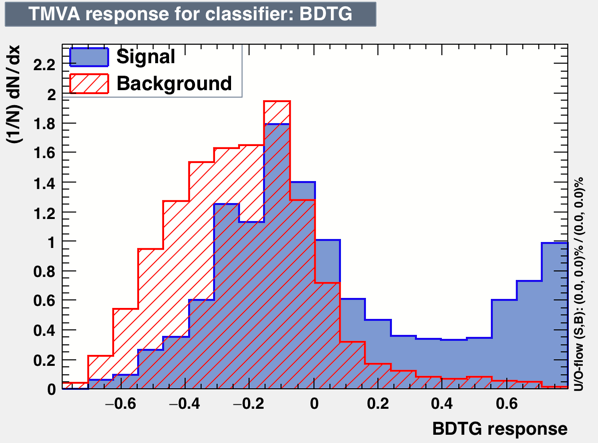
\includegraphics[scale=0.40]{Plots/BDT_Performance/Trial2/dataset/plots/mva_BDTG.png}%
	~
	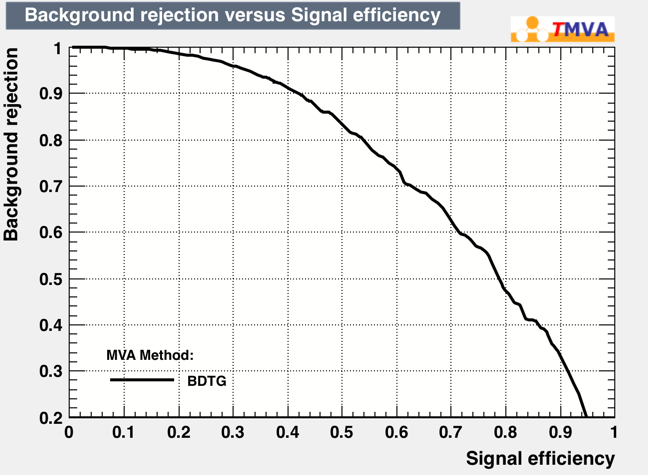
\includegraphics[scale=0.40]{Plots/BDT_Performance/Trial2/dataset/plots/rejBvsS.png}
	\caption{Left: BDT response for signal and background; Right: ROC curve}
\end{figure}

\begin{figure}[h!]
	 \centering
	 \subfigure[]{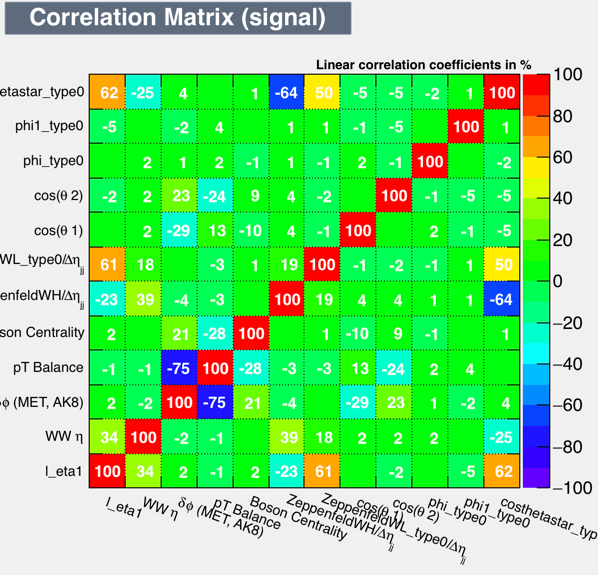
\includegraphics[width=1.2\textwidth, angle =90]{Plots/BDT_Performance/Trial2/dataset/plots/CorrelationMatrixS.png}}
	 \caption{Correlation plot for signal}
\end{figure}
\begin{figure}[h!]\ContinuedFloat
	 \subfigure[]{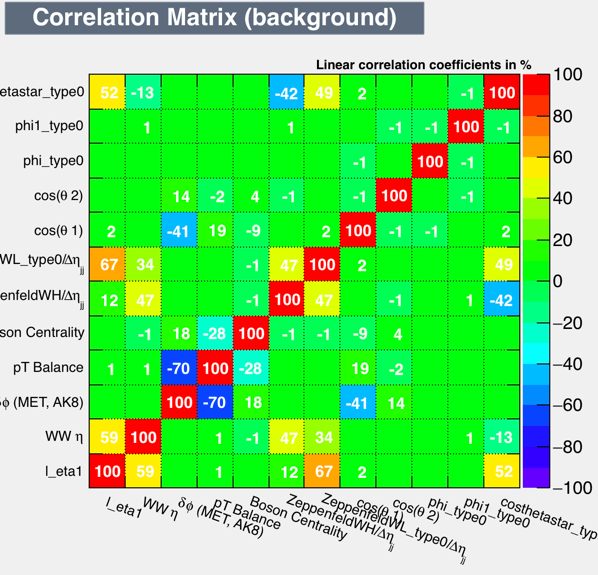
\includegraphics[width=1.2\textwidth, angle =90]{Plots/BDT_Performance/Trial2/dataset/plots/CorrelationMatrixB.png}}
	 \caption{Correlation plot for background}
\end{figure}

\subsubsection{Significance from combine}
The combine card is
\begin{verbatim}
----------------------------------------------------------
imax 1 number of channels
jmax * number of background
kmax * number of nuisance parameters
---------------------------------------------------------
shapes * * Nominal.root $PROCESS $PROCESS_$SYSTEMATIC
shapes data_obs * Nominal.root data
----------------------------------------------------------
Observation -1
bin WV WV WV WV WV
----------------------------------------------------------
process top W+jets Z+jets Diboson aQGC
process 1 2 3 4 0
rate -1.00000 -1.00000  -1.00000  -1.00000  -1.00000  
----------------------------------------------------------
lumi_13TeV			lnN	1.027	1.027	1.027	1.027	1.02700  
norm_Wjet 			lnN	-		1.100	-		-		-  
CMS_eff_b_mistag	lnN	0.980	0.980	0.98	0.980	0.98000
CMS_eff_m      		lnN	1.018	1.018	1.018	1.018	1.01800
CMS_eff_e      		lnN	1.017	1.017	1.017	1.017	1.01700
ewk_qqbar      		lnN	-		-		-		-		1.15000   
norm_top          	lnN	1.10	-		-		-		-  
----------------------------------------------------------
\end{verbatim}

Significance we get with BDT observable is 11.9113.

The distribution for the BDT observable is 
\begin{figure}[htb]
  \begin{center}
    \begin{tabular}{c}
    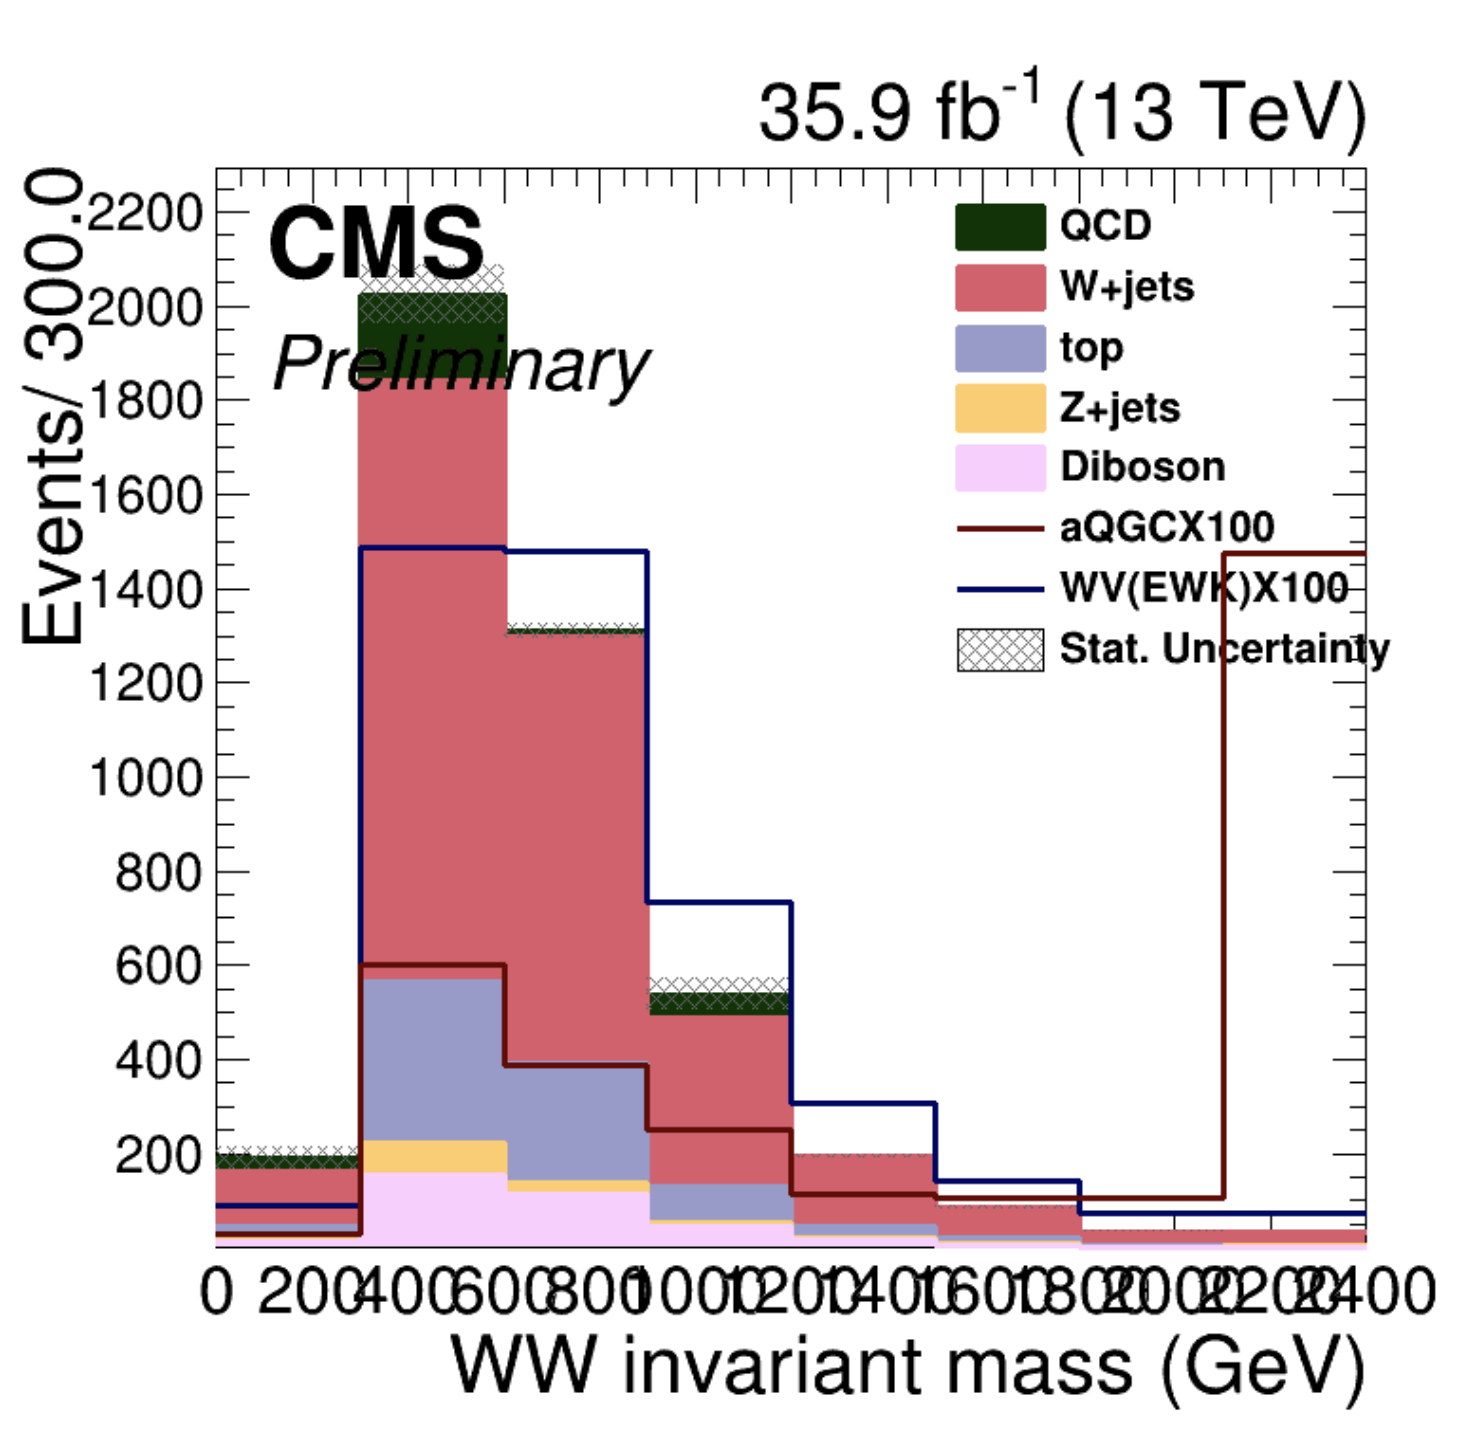
\includegraphics[width=0.90\textwidth]{Plots/BDT_Performance/Trial2/mWW.png}    
    \end{tabular}
    \caption{WW system invairant mass. This is our observable.}
    \label{fig:gen1}
  \end{center}
\end{figure}


\subsection{Cut Based Significance}
Cuts that we applied for cut based are:
\begin{itemize}
	\item Exactly one lepton having
	\begin{itemize}
		\item $p_T > 30$ GeV
		\item $|\eta| < 2.4$
	\end{itemize}
	\item pfMET $>$ 50 GeV
	\item AK8 jets
	\begin{itemize}
		\item  p$_T >$ 200 GeV
		\item $|\eta|<2.4$
		\item $\tau 21 < 0.55$
		\item 65$<$mW$<$105
	\end{itemize}
	\item Loose AK4 b-tagged jet veto
	\begin{itemize}
		\item $p_T>30$ GeV
		\item $\delta \eta > 4.0$
		\item $m_{jj}>900$ GeV
	\end{itemize}
	\item Boson centrality $<$ 0.3
	\item Leptonic and hadronic zeppenfeld $<$ 0.3
\end{itemize}

In this case our observable is again invariant mass of WW system (i.e. mWW). The distribution of mWW is:

\begin{figure}[htb]
  \begin{center}
    \begin{tabular}{c}
    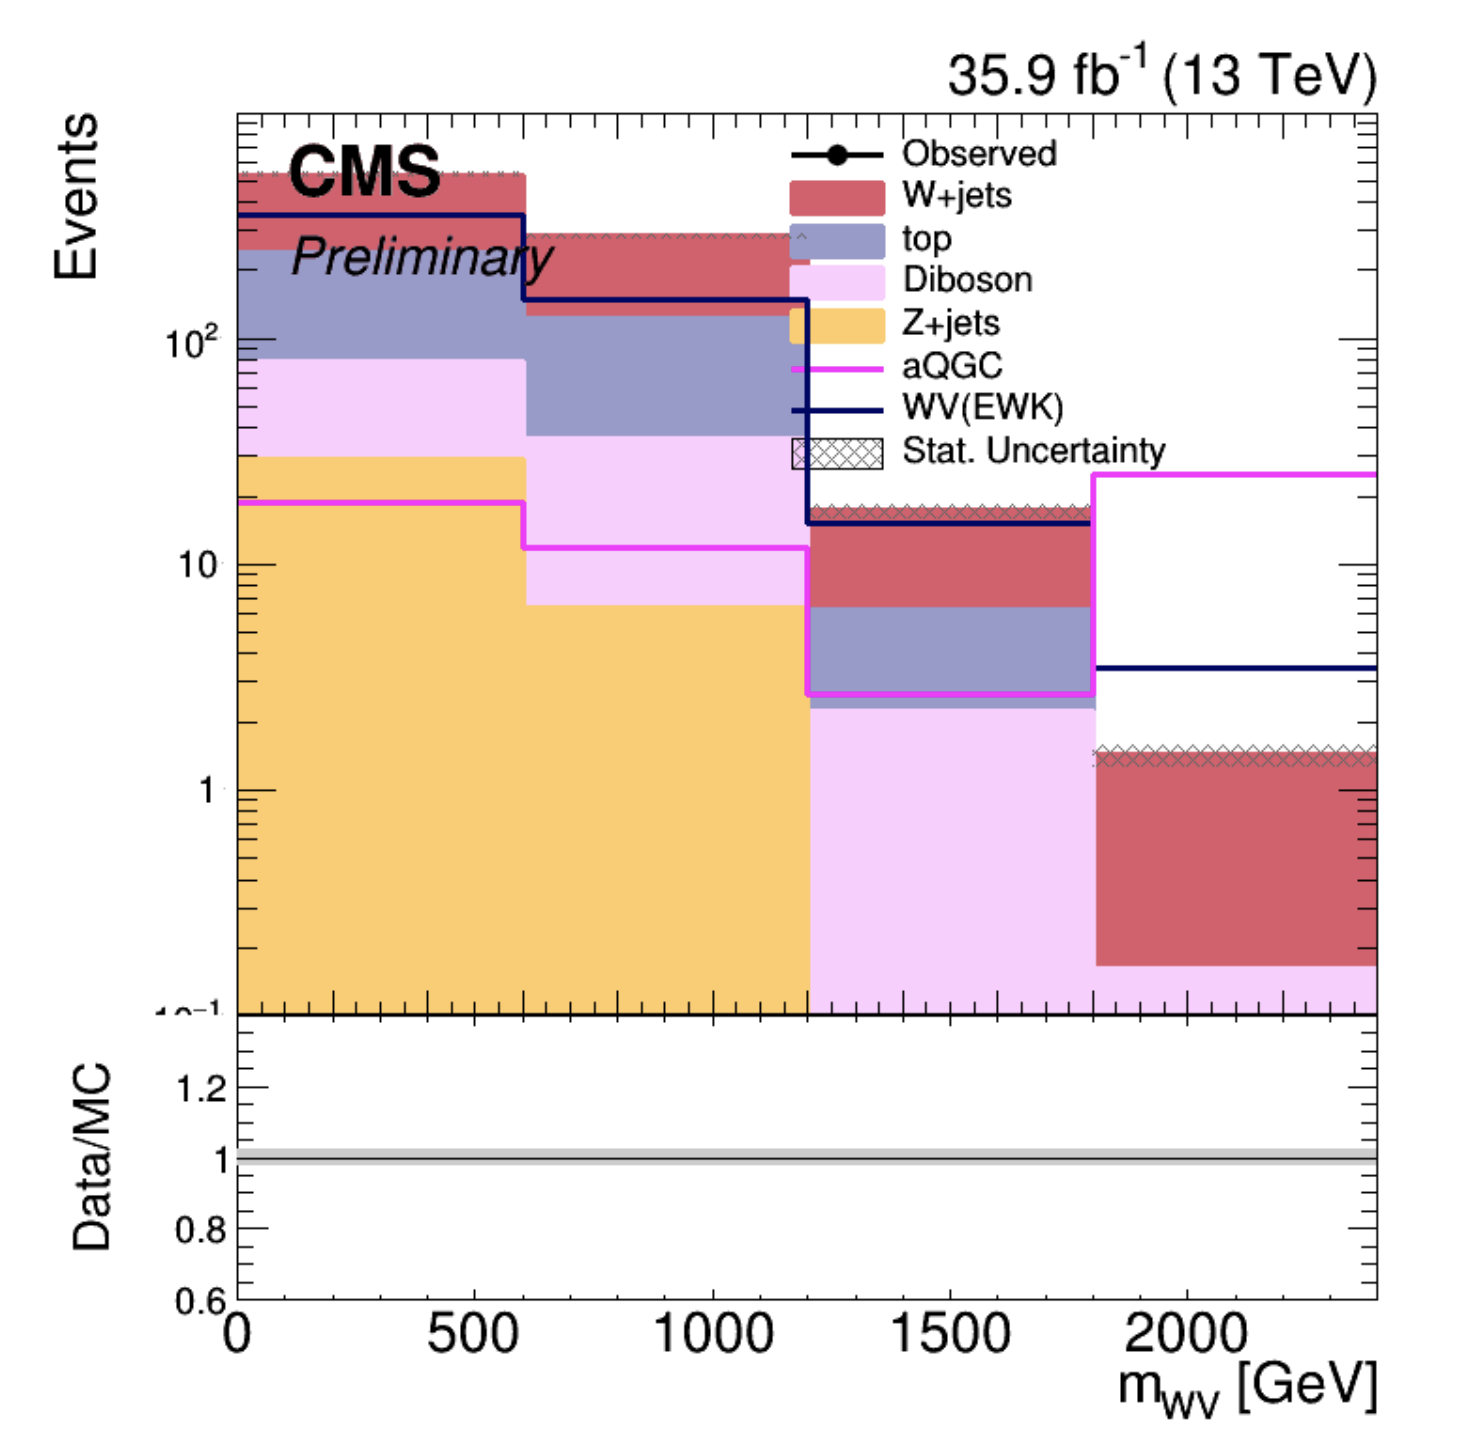
\includegraphics[width=0.90\textwidth]{Plots/BDT_Performance/mWW_CutBased.png}    
    \end{tabular}
    \caption{WW system invairant mass. This is our observable.}
    \label{fig:cutbasedObs}
  \end{center}
\end{figure}

The significance that we get with cut based is 10. THe combine card that we used is same as previous:
\begin{verbatim}
----------------------------------------------------------
imax 1 number of channels
jmax * number of background
kmax * number of nuisance parameters
---------------------------------------------------------
shapes * * Nominal.root $PROCESS $PROCESS_$SYSTEMATIC
shapes data_obs * Nominal.root data
----------------------------------------------------------
Observation -1
bin WV WV WV WV WV
----------------------------------------------------------
process top W+jets Z+jets Diboson aQGC
process 1 2 3 4 0
rate -1.00000 -1.00000  -1.00000  -1.00000  -1.00000  
----------------------------------------------------------
lumi_13TeV			lnN	1.027	1.027	1.027	1.027	1.02700  
norm_Wjet 			lnN	-		1.100	-		-		-  
CMS_eff_b_mistag	lnN	0.980	0.980	0.98	0.980	0.98000
CMS_eff_m      		lnN	1.018	1.018	1.018	1.018	1.01800
CMS_eff_e      		lnN	1.017	1.017	1.017	1.017	1.01700
ewk_qqbar      		lnN	-		-		-		-		1.15000   
norm_top          	lnN	1.10	-		-		-		-  
----------------------------------------------------------
\end{verbatim}

Thus, as we can see that we not not ganing anything with the multivariate analysis so we decided to move further with the cut based analysis.
